\documentclass{book}
\usepackage[hidelinks]{hyperref}
\usepackage{titlepic}
\usepackage{graphicx}
\usepackage{caption}
\usepackage{subcaption}
\usepackage{alltt}
\usepackage{fancyhdr}
\usepackage{minted}
\usepackage{exercise}
\usepackage{mathtools} 
\usepackage{csquotes}

\DeclareGraphicsExtensions{.pdf,.png,.jpg}
\DeclarePairedDelimiter\ceil{\lceil}{\rceil}
\DeclarePairedDelimiter\floor{\lfloor}{\rfloor}
\graphicspath{{./pics/}}
\setcounter{tocdepth}{4}
\renewcommand{\headheight}{0.6in}
\setlength{\headwidth}{\textwidth}

\fancyhead[L]{ % left
   
\includegraphics[height=0.53in]{logo}
}
\pagestyle{fancy}

\begin{document}

\title{Machine learning for bio-image analysis}

\author{Cedric Hassen Khodja \and Jean-Bernardand Fiche \and  Volker Baecker \\ \small Montpellier Ressources Imagerie}

\date{17.01.2019}

\titlepic{
    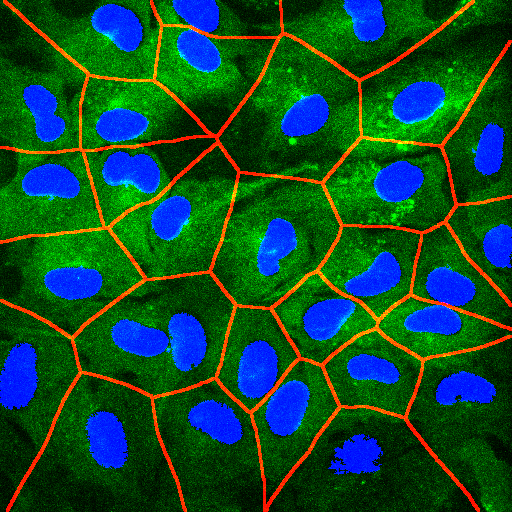
\includegraphics[width=\textwidth, height=3.2in]{title}
    }

\maketitle
\tableofcontents
\listoffigures
\chapter{Introduction}

In a scratch assay a gap in a tissue is produced with the tip of a pipette. Images of the tissue are taken in regular time intervals. The relative area of the gap for each time--point is then measured to analyze the speed with which the gap is closing.  

\begin{figure}[!htb]
 \centering
 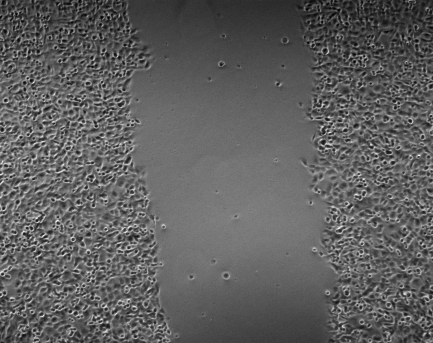
\includegraphics[width=8cm]{scratch_assay}
 \caption{An image from sratch assay analysis.}
 \label{figure:scratch-assay}
\end{figure}

In this exercise you will try to segment the gap first using image analysis with FIJI/ImageJ and the using machine learning with Ilastik.

\section{Image Analysis, Features and Scalespace}

Run {\tt FIJI} and open one of the images from the folder {\tt ex01-scratch-assay}.

\begin{figure}[!htb]
 \centering
 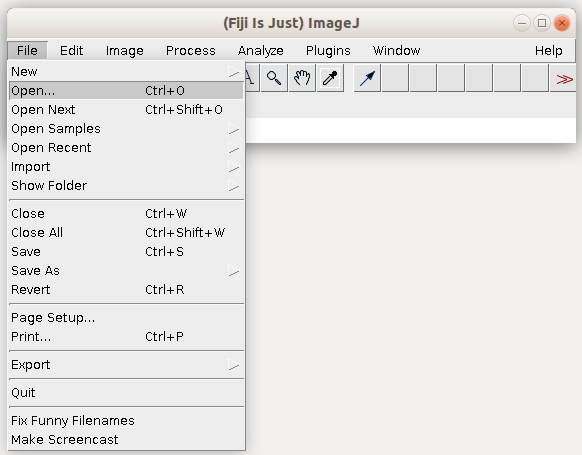
\includegraphics[width=8cm]{fiji_open_image}
 \caption{Opening an image in FIJI.}
 \label{figure:fiji-open-image}
\end{figure}

Try to segment the gap and measure its area! Hint: You find some ImageJ commands you might need below.

\subsection{ImageJ commands you might need}

\begin{description}
 \item[Image \textgreater Adjust \textgreater Threshold...] \hfill \\ 
 Create a binary mask from the image.
 \item[Process \textgreater Filters \textgreater Variance...] \hfill \\ Create a new image in which each pixel is replaced with with the variance in a local neighborhood.
 \item[Process \textgreater Find Edges (Sobel filter)] \hfill \\ An edge detector using a combination of convolution filters.
 \item[Process \textgreater Filters \textgreater Gaussian Blur...] \hfill \\ A convolution filter using a Gaussian distribution as kernel. Using a small width of the Gaussian, high frequencies are removed from the image, bigger widths remove lower frequencies. Applying a Gaussian filter with a given width, corresponds to choosing a point in the scale space.
\item[Analyze \textgreater Measure] \hfill \\
Measure the current image or selection. 
\end{description}

The plugin {\tt FeatureJ} provides further features. The selection of a scale, i.e. the application of a Gaussian Blur filter is integrated for the commands of this plugin. The commands of this plugin can be run from a panel that can be opened from {\tt Plugins \textgreater FeatureJ \textgreater FeatureJ Panel}.

\begin{figure}[!htb]
 \centering
 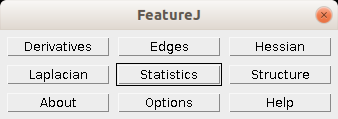
\includegraphics[width=6cm]{featurej_panel}
 \caption{The FeatureJ command-panel.}
 \label{figure:featurej}
\end{figure}

\begin{description}
 \item[Derivatives] \hfill \\ 
 Create an image containing the change (or the change of the change, ...) of the intensities in a given direction.
 \item[Edges] \hfill \\
 A canny edge detector.
 \item[Hessian] \hfill \\
 Creates an image based on the second order partial derivatives of the original image. It can be used to distinguish between plate-like, line-like and blob-like structures.
 \item[Laplacian] \hfill \\
 Creates an image based on the sum of the second order partial derivatives of the image. It is often used for edge and for blob detection. The Laplacian can be implemented as a convolution filter.
 \item[Statistics] \hfill \\
 This command does not create a feature but calculates statistics on an image or a selection. The values calculated can be used to classify objects that have been segmented before.
  \item[Structure] \hfill \\
Creates an image based on the structure tensor which represents the distribution of the gradient directions. It can be used to segment images based on texture.
\end{description}

\section{Machine Learning}

You will now use machine learning to do the segmentation of the gap-area in the scratch assay analysis. 

\begin{enumerate}
\item Start Ilastik and create a new pixel classification project.
\item Add a new (separate) image from the folder {\tt ex01-scratch-assay} to the project.
\begin{figure}[!htb]
 \centering
 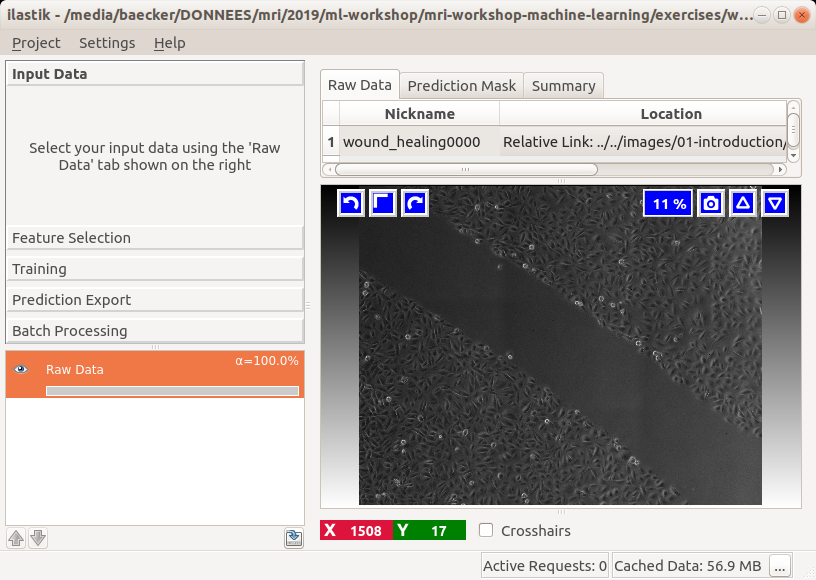
\includegraphics[width=8cm]{ilastik}
 \caption{Image import into Ilatik.}
 \label{figure:ilastik}
\end{figure}
\item Adjust the zoom, so that the whole image is visible.
\item Advance to the {\tt Feature Selection} step, open the {\tt Feature Selection Dialog} and select all features on all scales. Also add a new scale of your choice, bigger than the ones initially proposed. We will refine the feature and scale selection later.
\item Close the {\tt Feature Selection Dialog} and click on different features at different scales in the features--list. Which features at which scales do you think are the most useful for the segmentation of the gap? Note the 2 most useful features with their scales:
\begin{verbatim}
Feature 1:


Scale of feature 1:

Feature 2:


Scale of feature 2:

\end{verbatim} 
\item Advance to the {\tt Training} step. Rename the classes for the pixel-classifiction from {\tt Label 1} to {\tt tissue} and from {\tt Label 2} to {\tt gap}. Change the colors of the classes from yellow and blue to red and green.

\item Select the {\tt tissue} class and draw 3 or 4 strokes on the tissue using the brush--tool. Then select the {\tt gap} class and draw 3 or 4 strokes in the gap. Press the {\tt Live Update} button to see the result of the segmentation.

\item If necessary add more strokes for the two classes with the brush--tool or remove strokes using the eraser--tool. The segmentation will be updated immediately as long as the {\tt Live Update} is active.

\item Deactivate the {\tt Live Update} and advance to the {\tt Prediction Export}. Export the segmentation into a {\tt .tiff}--file. You need to select the right {\tt Source} and the right image file-format from the {\tt Choose Export Image Settings} dialog. Then press the {\tt Export All}--button.

\item Open the exported segmentation--image with {\tt Fiji}. The values in the image correspond to the indexes of the classes. In this case they are 1 and 2. Use the threshold-adjuster to create a mask. Run the {\tt fill-holes} command. Use the particle--analyzer to add a selection of the gap to the {\tt roi-manager} and measure the surface of the gap.
\begin{verbatim}
Name of the image:

area of the gap [pixel]: 
\end{verbatim}
\item Go back to {\tt Ilastik} and advance to the {\tt Batch Processing} step. Select some of the images not yet processed, from the folder {\tt ex01-scratch-assay}. Run the segmentation on the input files and control the results with {\tt Fiji}.

\item Open a segmentation--result, create a {\tt ROI} from the selection and display it on the original input image. How good is the segmentation? Does it correctly reflect the borders of the gap/tissue?
\begin{figure}[!htb]
 \centering
 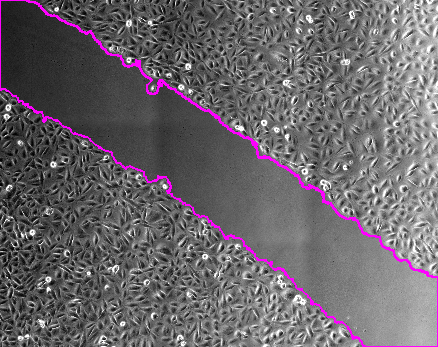
\includegraphics[width=8cm]{wound_healing_result}
 \caption{The ROI of the segmentation displayed on the input image.}
 \label{figure:ilastik-segmentation-result}
\end{figure}

\end{enumerate}
\chapter{Introduction to Machine Learning}

\begin{displayquote}
''Machine learning algorithms build a mathematical model of sample data, known as "training data", in order to make predictions or decisions without being explicitly programmed to perform the task.''\cite{wiki:machine_learning_2019}
\end{displayquote}

Machine learning is a sub--field of artificial intelligence. It is closely related to statistics, statistical learning, data--mining and optimization. A number of machine learning applications are today in use on a regular basis. Machine learning is for example used in 

\begin{itemize}
\item speech recognition
\item image recognition 
\item spam filtering
\item medical diagnosis
\item games: chess, checkers, go
\item price prediction
\item recommendation of products
\item self-driving cars 
\item fraud-detection
\end{itemize}

In bio--image analysis classical machine learning (as opposed to deep-learning) is for example used for:

\begin{itemize}
\item pixel classification (segmentation)
\item cell counting
\item object classification (types of cells)
\item tracking
\item Interactive 3D Segmentation (carving)
\item Boundary-based segmentation with Multicut
\end{itemize}

Deep learning is a special form of machine learning that we will treat in the second part of this course. More recently deep--learning is applied to solve bio-image analysis problems. Besides applications already listed for classical machine learning, some examples are:

\begin{itemize}
\item image restoration
\item prediction of distance maps
\item predict high-resolution images from a low-resolution images in SRLM
\item segmentation of bacteria cells 
\end{itemize}


%\input{recall-classical-bio-image-analysis}
%\input{pixel-classification}
%\input{object-classification}
%\input{object-counting}
%\input{special applications}

\bibliographystyle{plain}
\bibliography{workshop}
\end{document}